\documentclass[12pt]{article}
\usepackage{graphicx}
\usepackage{wrapfig}
\usepackage{subfigure}
\usepackage{multirow}
\usepackage{hyperref}
\usepackage{amsmath}
\usepackage{amssymb}
%\usepackage{ngerman}
\usepackage[ansinew]{inputenc}
\usepackage[left=2cm,top=1cm]{geometry}

% vector graphics test
\usepackage{color}
\usepackage{transparent}
\graphicspath{{graphs/}}





\begin{document}
	\pagestyle{empty}


\begin{titlepage}
    \centering
	\huge{Constructing the Equation of State for Compact Stars}\\
	\bigskip
    \large{Bachelor thesis}\\
    \huge{Jan R\"{o}der}
\end{titlepage}

%headline!!!


\tableofcontents
\pagebreak


\section{Introduction}

To this day, the nature of the equation of state [EOS] for neutron stars is highly debated. Previously discussed EOSs have emerged from
various topics and models of physics. Each one has different parameters determining its impact on calculations. \\
For the past years, it has been common to derive an EOS from a theory and then use it to construct a mass-radius relation [MRR]. This method is obviously constrained by the fact that one cannot put an arbitrary number of theories into one EOS. That would result in a problem impossible to solve, even for computers. Therefore, the motivation is to minimize the number of parameters and constraints in the future.\\
The approach chosen in this thesis is inverting the above process. Instead of using an EOS to calculate masses and radii, those shall now take over the role as input parameters. For compact stars up to a certain mass, the EOS will be assumed to be known well enough. Above that mass a numerical reconstruction will take place, determining the EOS from a variety of MRRs. 


\pagebreak
\section{Preparations}

\subsection{The Tolman-Oppenheimer-Volkoff equation}

Before getting into the actual method, a theoretical basis has to be set up.
This involves a derivation of the equation used for determining the structure of compact stars. Here, that will be the 
Tolman-Oppenheimer-Volkoff [TOV] equation. \\
To make analytical and numerical calculations easier, the unit system is chosen to be $c=G=1$, so that every unit is a 
power of length.\\
The derivation is based off the assumption that the star matter can be described as a perfect/ideal fluid. 
Further, the system shall not evolve in time, therefore staying spherically symmetric. In terms of the energy-momentum tensor we are left with:

\begin{equation}\label{eq:hydro}
	T_{\mu\nu}=\left(\epsilon + P\right)u_\nu u_\mu-Pg_{\mu\nu}
\end{equation}
Spherical symmetry leads to a certain form of the metric, which then gives the stress-energy tensor components:
\begin{equation}
	T_{\mu\nu} = diag(\epsilon e^{\nu(r)}  , \ P e^{\lambda(r)},\ Pr^2,\ Pr^2sin^2(\theta)    )
\end{equation}
Imposing hydrostatic equilibrium,
\begin{equation}
	\nabla_\nu T^{\mu\nu}=0
\end{equation}
and some calculation, one obtains the expression
\begin{equation}
	content...
\end{equation}
To determine what $\nu(r)$ looks like, and using the previously defined metric, one can calculate the non-zero components
of the Ricci tensor:
\begin{equation}
	content...
\end{equation}
The Einstein equations then yield more equations containing $\nu(r)$ and it's derivatives. After plugging some of the equations 
into one another, one obtains $\nu(r)$ and therefore, in conclusion, the full TOV equation:
\begin{equation}\label{eq:tov}
	\frac{dP}{dr} = \frac{(\epsilon + P)(m + 4\pi r^3 P)}{2mr-r^2}
\end{equation}
Together with a second equation for the mass:
\begin{equation}\label{eq:mr}
	\frac{dm}{dr} = 4\pi r^2\epsilon
\end{equation}

\subsection{Numerical solution}

\subsubsection{Method}

The TOV equations come in the form of a first-order ordinary differential equation system (ODE). In order to obtain sufficient precision, a 4th-order Runge-Kutta algorithm shall be used to solve said ODE. By looking at both equations, our ODE system is given in the form:
\begin{equation}\label{eq:ode}
	\dot{y}(t) = f(y(t), t)
\end{equation}
where $\dot{y}(t)$ is a two component "vector":
\begin{equation}
	\dot{y}(t) =  \left( \begin{array}{c}dP/dr\\dm/dr\end{array} \right)
\end{equation}
$f(y(t), t)$ then contains the right hand side of equations \ref{eq:tov} and \ref{eq:mr}. \\
Numerically, solving the ODE is achieved by approximation of a step $\tau$ in the function variable $t$ (in TOV, this is the radius $r$) with derivatives of the function that is the ODE solution ($y$). 
\begin{equation}
	y(t+\tau) = y(t) + \frac{1}{6} (k_1 + 2k_2 + 2k_3 + k_4)
 \end{equation}
with increments $k_i$:
\begin{align*}
	k_1 &= f(y(t),t)\cdot\tau\\
	k_2 &= f(y(t)+k_1/2,t+\tau/2)\cdot\tau\\
	k_3 &= f(y(t)+k_2/2,t+\tau/2)\cdot\tau\\
	k_4 &= f(y(t)+k_3,t+\tau)\cdot\tau
\end{align*}
All $k_i$ are of course also two component "vectors". 

\subsubsection{Adaptive stepsize}

In order to maintain a minimum level of precision, the program checks for the change in pressure resulting from one Runge-Kutta step. If said change is too large, the step size $\tau$ is varied by a factor and the Runge-Kutta step count is reduced by one. Upon repeating the step, the same check takes place, and if necessary another $\tau$ adjustion. If the check is successful, the program will accept the step result and proceed with the next one. 

\subsubsection{Implementation}

In the actual program (written in C), the left hand side of our ODE system is implemented as a two-dimensional array of form y[N][x]. 
N will be two, for the whole program, as we will not add other equations to the system. The $k_i$ are all one-dimensional arrays; that way $x$ is only reflecting the step count. $x$ will therefore be in range zero up to the number of iteration steps. We set an arbitrary maximum step amount to prevent segmentation faults.







\section{Basic algorithm}


The goal is to reconstruct the EOS with as few biasing and imposing of mathematical form as possible. Therefore, the only pre-determined input is an EOS corresponding to a given mass in the MRR (Fig. \ref{fig:mce}). From there, the EOS can be constructed without further constraint. Here, a straight line is added to the end of the EOS, that is, in the high density region (Fig. \ref{fig:recon} b). The ODE solver starts at a point near the end of the given EOS and will calculate a mass with the (now small) piece of straight line and the EOS. If the mass does not fit the corresponding one in the MRR that was read in previously, the starting point on the line will be shifted to a higher pressure by a small step. At some very high pressure, a cut-off can be applied due to un-physical energy densities. If the starting point reaches the cut-off and the correct mass was not found, the slope of the line is varied. The process then starts over at a point near the given EOS and shifting stepwise from there (Fig. \ref{fig:recon} c).

\begin{figure}
	\centering
	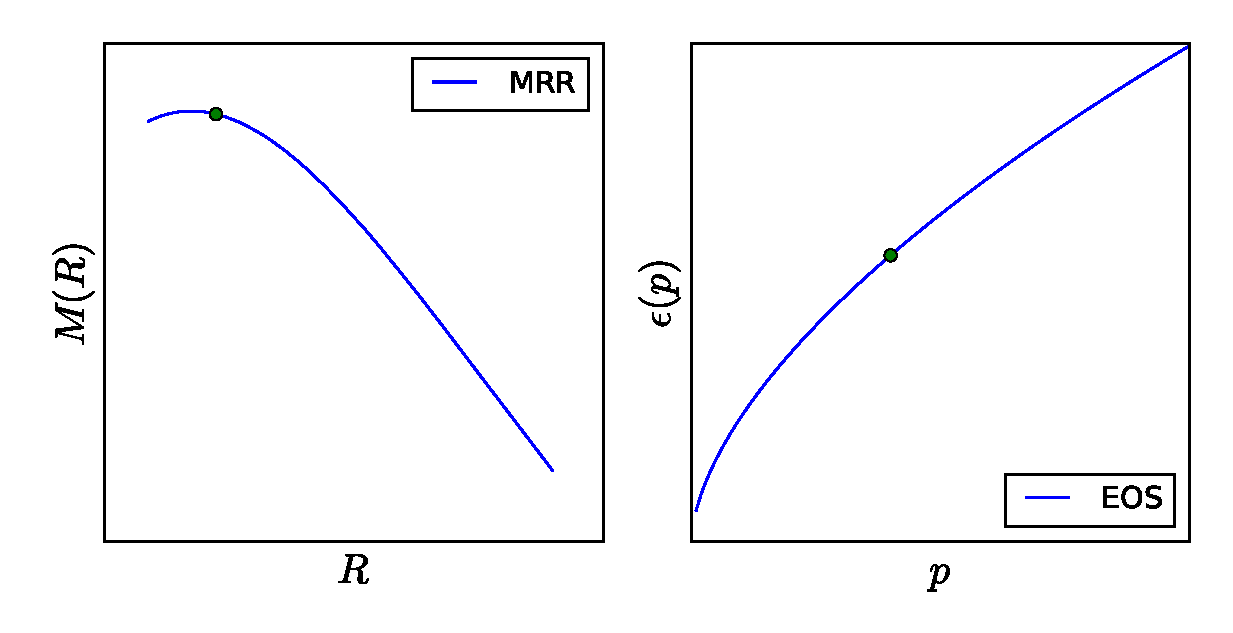
\includegraphics[width=1\textwidth]{graphs/mrr_corr_eos}
	\caption{corresponding points in MRR and EOS. Point in EOS resembles values in the center of the star.}
	\label{fig:mce}
\end{figure}


\begin{figure}
	\centering
	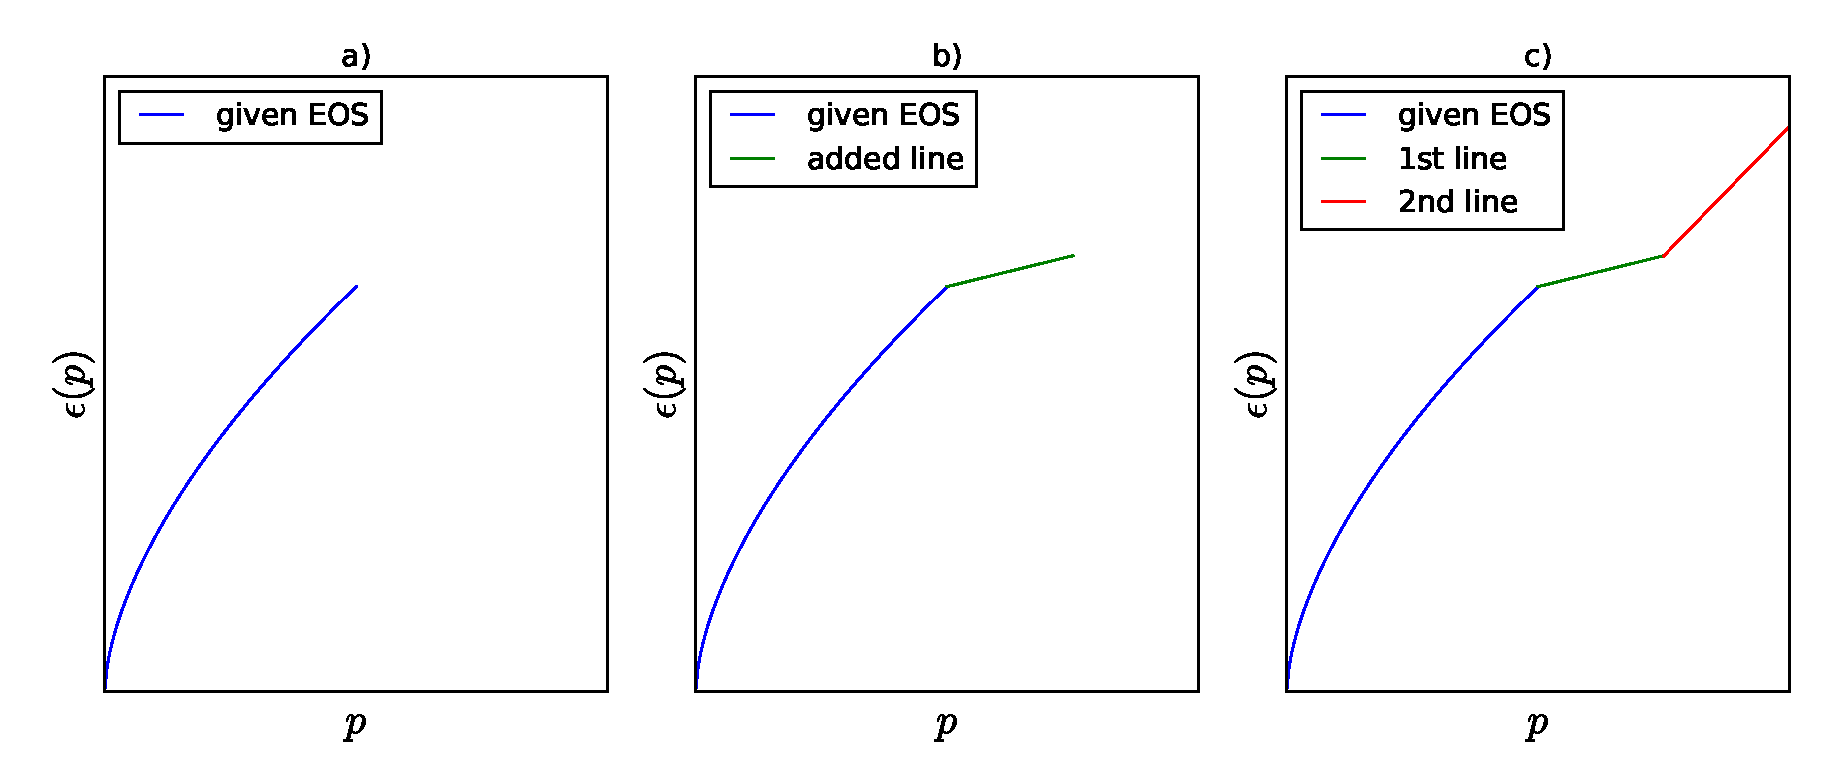
\includegraphics[width=1\textwidth]{graphs/eos_recon}
	\caption{a) Given polytropic equation of state, b) added a constructed straight line, c) added another line, in calculations, the green one will be used as part of the EOS}
	\label{fig:recon}
\end{figure}











\pagebreak

%%%ALTERNATIVE BILDUMGEBUNG
% \begin{figure}[h]
% \begin{center}
% \includegraphics[width=50mm]{fig1}
% \caption{Fadenpendel \cite{Eichler}.}\label{fig:1}
% \end{center}
% \end{figure}




\hspace{15pt}

\begin{table}[h!]
  \centering
  %\caption{Caption for the table.}
  \label{tab:2}
  \begin{tabular}{|c||c|}
  \hline
    Messung der Fadenl�nge & $l$ (m)\\
    \hline\hline
    1 &   \\ \hline
    2 &   \\ \hline
    3 &   \\ \hline
    4 &   \\ \hline
    5 &   \\ \hline
    Mittelwert $\bar{l}$ &  \\ \hline
    Standardabweichung $\sigma_l$ &  \\ \hline
  \end{tabular}
\end{table}



\begin{thebibliography}{2}
%\bibitem{Eichler} H. J. Eichler, H.-D. Kronfeldt, J. Sahm, \textit{Das Neue Physikalische Grundpraktikum}, Springer-Verlag, Berlin-Heidelberg, 2001.
%\bibitem{Kuchling} H. Kuchling, \textit{Taschenbuch der Physik, 21. Auflage}, Fachbuchverlag Leipzig, 2014.
\end{thebibliography}

\end{document}